\documentclass[../main/main.tex]{subfiles}
\graphicspath{{./figures/}}

\makeatletter
\renewcommand{\@chapapp}{Travaux pratiques -- TP}
\makeatother

\toggletrue{student}
\HideSolutionstrue
\toggletrue{corrige}
% \renewcommand{\mycol}{black}
\renewcommand{\mycol}{gray}

\begin{document}
\setcounter{chapter}{10}

\chapter{Cin\'etique d'une r\'eaction de saponification par conductim\'etrie}

\enonce{
	\begin{prgm}
		\begin{tcb}*(ror)"know"{Savoirs}
			\begin{itemize}[label=$\diamond$, leftmargin=10pt]
				\item Relever les indications sur le risque associé au prélèvement, au
				      mélange et au stockage des produits chimiques et adopter une attitude
				      responsable lors de leur utilisation.
				\item Suivi cinétique de transformations chimiques.
				\item Suivi en continu d'une grandeur physique.
			\end{itemize}
		\end{tcb}
		\begin{tcb}*(ror)"how"{Savoir-faire}
			\begin{itemize}[label=$\diamond$, leftmargin=10pt]
				\item Établir une loi de vitesse à partir du suivi temporel d’une
				      grandeur physique.
				\item Exploiter les résultats d’un suivi temporel de concentration pour
				      déterminer les caractéristiques cinétiques d’une réaction.
				\item Proposer et mettre en œuvre des conditions expérimentales
				      permettant la simplification de la loi de vitesse.
				\item Déterminer la valeur d’une énergie d’activation.
			\end{itemize}
		\end{tcb}
	\end{prgm}
	\vspace{-10pt}
	\section{Objectifs}
	\begin{itemize}
		\item Utiliser une méthode conductimétrique pour vérifier un ordre global et
		      pour déterminer la valeur d'une constante de vitesse $k$.
		\item Se placer dans des conditions expérimentales de proportions
		      stœchiométriques.
		\item Déterminer une énergie d'activation.
	\end{itemize}
}

\enonce{%
	\section{S'approprier}
	\subsection{Introduction}

	La réaction de saponification est l'hydrolyse basique (en présence d'ions
	$\ce{OH^-}$) des esters, cette réaction permet la synthèse des savons. Le savon,
	produit domestique utilisé depuis des milliers d'années est à l'origine un
	mélange de graisse animale fondue et de cendres. En 1823, Eugène
	\textsc{Chevreul}, chimiste français, découvre que les triesters présents dans
	les corps gras, réagissent avec la soude (base qui était jadis apportée par les
	cendres) pour former le savon.

	\subsection{Le principe de la conductimétrie}

	% Cette méthode repose sur l'existence d'ions en solution et sur leur capacité à
	% faciliter le passage d'un courant. La nature des ions et leurs concentrations
	% modifient la conductance $G$ du système (grandeur qui est l'inverse de la
	% résistance $R$) exprimée en \si{S} (Siemens). Plus le milieu est propice au
	% passage du courant, plus la conductance est élevée. Celle-ci est reliée à trois
	% paramètres principaux~:
	%
	% \begin{enumerate}
	% 	\item la conductivité $\sigma$ du système
	% 	\item la longueur $\ell$
	% 	\item la section $S$ de la cellule
	% \end{enumerate}
	%
	% La conductance s'exprime alors selon
	% \[G = \frac{\sigma S}{\ell}\]
	%
	% Ainsi, on ne parle pas de conductance \cancel{de la solution}, puisque la
	% conductance dépend de la cellule de mesure et de sa géométrie. L'unité de
	% conductivité est le $\si{S.m^{-1}}$~; le quotient $K = \ell / S$ est appelé
	% constante de cellule. Ainsi, on a $G = \sigma / K$. La mesure de la conductance
	% s'effectue avec un conductimètre, qui est en fait un ohmmètre.\bigbreak

	La conductivité $\sigma$ de la solution peut s'exprimer par la \textbf{loi
		de Kohlrausch}, exprimée sous une forme avec la chage de l'ion~:
	\begin{tcb}(prop)'l'{Loi de \textsc{Kohlrausch}}
		\[\boxed{\sigma = \sum_{i} \lambda_i \left|z_i\right| [{\rm X}_i]}\]
		\begin{itemize}
			\item $\lambda_i$ la conductivité molaire ionique de l'ion ${\rm X}_i$ (en
			      $\si{S.m^2.mol^{-1}}$) donnée dans les tables
			\item $z_i$ la charge de l'ion ${\rm X}_i$
			\item $[{\rm X}_i]$ la concentration de l'ion ${\rm X}_i$
		\end{itemize}
	\end{tcb}

	\begin{tcb}(impo)'l'{Important}
		\begin{center}
			\bfseries
			La conductivité $\sigma$ de la solution prend en compte tous les ions
			présents dans la solution. Il faut donc faire l'inventaire des ions en
			solution avec soin.
		\end{center}
	\end{tcb}

	% En supposant que l'on ne fait varier que d'une unique espèce ionique (et donc
	% conductrice) dans la solution, on pourra noter $c = [{\rm X}_i]$ la
	% concentration de cette espèce. La \textbf{courbe d'étalonnage} est alors la
	% représentation graphique de $\sigma = f(c)$ obtenue avec l'ensemble des points
	% de coordonnées $(c_i~; \sigma_i)$ où $\sigma_i$ sont les conductivités des
	% différentes solutions étalons $S_i$ de concentration $c_i$. Connaissant la
	% conductivité $\sigma_0$ de la solution $S_0$ inconnue, on en déduit grâce à la
	% courbe d'étalonnage la concentration molaire $c_0$ de la solution $S_0$.
}

\setcounter{section}{2}
\section{Analyser}
\enonce{%
	\subsection{Données numériques utiles}

	\begin{tcb}(data)<lfnt>'l'{Données}
		\begin{minipage}{0.50\linewidth}
			\centering
			\begin{tabular}{lccc}
				\toprule
				Ions                     &
				\ce{HO-}                 &
				\ce{CH3CO2-}             &
				\ce{Na+}                   \\
				$\lambda$ \newline
				($\si{mS.m^2.mol^{-1}}$) &
				\num{19.86}              &
				\num{4.09}               &
				\num{5.01}                 \\
				\bottomrule
			\end{tabular}
		\end{minipage}
		\begin{minipage}{0.50\linewidth}
			\centering
			\begin{tabular}{lcccc}
				\toprule
				Élément                         & Na & C & O & H \\
				Masse molaire (\si{g.mol^{-1}}) &
				23                              &
				12                              &
				16                              &
				1                                                \\
				\bottomrule
			\end{tabular}
		\end{minipage}
		\begin{itemize}
			\item Densité de l'éthanoate d'éthyle pur~: $d = \num{0.90}$~;
			\item Constante des gaz parfaits~: $R = \SI{8.314}{J.K^{-1}.mol^{-1}}$
		\end{itemize}
	\end{tcb}
}
\setcounter{subsection}{1}

\subsection{Préliminaires}

\enonce{%
	La réaction étudiée ici est la saponification de l'éthanoate d'éthyle par la soude à température ambiante. C'est une réaction \textbf{totale et lente}.

	\begin{center}
		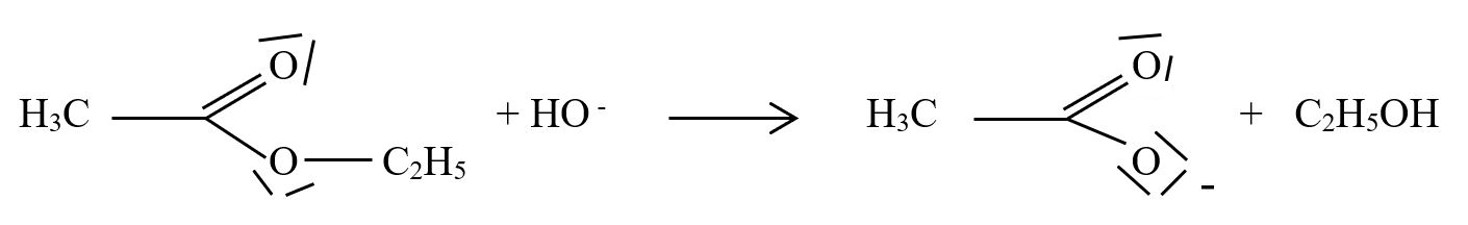
\includegraphics[width=0.7\textwidth]{reaction}
	\end{center}

	Par souci de simplicité, on notera par la suite la réaction~: \hfill
	\fbox{$\ce{RCOOR}'+\ce{OH^-} \rightarrow \ce{RCOO^-} + \ce{R}'\ce{OH}$}
}

\subsubsection{Rappels de chimie organique}

\setlist[blocQR,1]{leftmargin=10pt, label=\clenumi}
\QR{%
	Quelle est la classe fonctionnelle (ou famille) de l'éthanoate
	d'éthyle~? Quelle est son groupe caractéristique~? Quelle est sa formule
	semi-développée~? Nommer les deux produits obtenus.
}{%
	C'est un ester. Son groupe caractéristique est \ce{-COOR}. Sa formule
	semi-développée est \ce{CH3-CO2-C2H5}. Les deux produits obtenus sont
	l'éthanoate de sodium et l'éthanol.
}

\subsubsection{Choix de la méthode d'étude}
\QR{%
	Justifier que la conductimétrie soit une méthode particulièrement
	adaptée pour le suivi cinétique de cette réaction.
}{%
	On a une évolution des ions en solution~: on perd 1 ion \ce{HO-} et on gagne 1
	ion éthanoate. Comme leurs conductivités molaires sont différentes, on peut
	aisément suivre l'évolution de la réaction par ce biais.
}

\subsubsection{Sécurité}

\QR{%
	\begin{minipage}[t]{0.65\linewidth}
		On peut voir ces pictogrammes sur les étiquettes des flacons~: que
		signifient-t-ils~? quelles précautions faut-il prendre~?
		Vous pourrez consulter\\
		\url{http://www.inrs.fr/media.html?refINRS=ED\%204406}
	\end{minipage}
	\hfill
	\begin{minipage}[t]{0.30\linewidth}
		\vspace{0pt}
		$\underset{\text{Soude}}{\ghspic{acid}}$
		$\underset{\text{Éthanoate d'éthyl}}{\ghspic{flame}\ghspic{exclam}}$
		% \begin{center}
		%   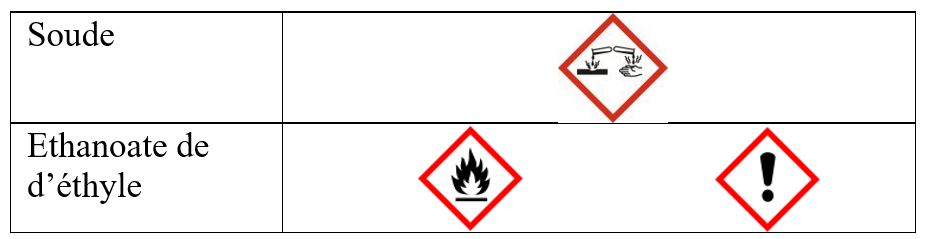
\includegraphics[width=\linewidth]{picto}
		% \end{center}
	\end{minipage}
}{%
	\ifstudent{
		~
	}
	\begin{tasks}(3)
		\task[\hspace*{2.5cm}\ghspic{flame}]\\
		Inflammable~: stockage et loin des flammes.
		\task[\hspace*{2cm}\ghspic{acid}]\\
		Ronge~: gants et lunettes.
		\task[\hspace*{2cm}\ghspic{exclam}]\\
		Danger pour santé ou ozone~: gants.
	\end{tasks}
}

\subsection{\'Etude théorique de la cinétique}

\enonce{%
	On cherche à vérifier que cette réaction est d'ordre global 2 avec un ordre
	partiel de 1 par rapport à chacun des réactifs.
}

\QR{%
	Écrire la loi de vitesse correspondante.
}{%
	\[
		v = k [\ce{RCOOR}'][\ce{HO-}]
	\]
}

\QR{%
Les conditions expérimentales sont choisies pour que l'on soit dans
les proportions stœchiométriques. De plus à l'instant initial, il n'y a
pas encore de produits. Ainsi,
\[[\ce{RCOOR}']_0 = [\ce{OH-}]_0 = c_0 \qet [\ce{RCOO-}]_0 =
	[\ce{R}'\ce{OH}]_0 = 0\]
Simplifier, dans ces conditions, la loi de vitesse précédente.
}{%
Avec $[\ce{RCOOR}'](t) = [\ce{HO-}](t) = c_0-x$, on a
\[
	\boxed{v = k(c_0-x)^{2}}
\]
}

\QR{%
	Faire un tableau d'avancement sur les concentrations aux instants $t =
		0$, $t$ quelconque, et $t\to \infty$ (noté $t_\infty$) sachant que la
	réaction est supposée \textbf{totale}. On introduira pour plus de
	commodité d'écriture $x$ l'avancement volumique $x = \xi / V$.
}{%
	~
	\begin{center}
		\def\rhgt{0.35}
		\centering
		\begin{tabularx}{\linewidth}{|l|c||YdYdYdY||Y|}
			\hline
			\multicolumn{2}{|c||}{
				$\xmathstrut{\rhgt}$
			\textbf{Équation}} &
			$\ce{RCOOR}'$      & $+$              &
			$\ce{HO-}$         & $\ra$            &
			$\ce{RCOO-}$       & $+$              &
			$\ce{R}'\ce{OH}$   &
			$\ce{Na+}$                              \\
			\hline
			$\xmathstrut{\rhgt}$
			Initial            & $x = 0$          &
			$c_0$              & \vline           &
			$c_0$              & \vline           &
			$0$                & \vline           &
			$0$                &
			$c_0$                                   \\
			\hline
			$\xmathstrut{\rhgt}$
			Interm.            & $x$              &
			$c_0 - x$          & \vline           &
			$c_0 - x$          & \vline           &
			$x$                & \vline           &
			$x$                &
			$c_0$                                   \\
			\hline
			$\xmathstrut{\rhgt}$
			Final              & $x_f = x_{\max}$ &
			$0$                & \vline           &
			$0$                & \vline           &
			$c_0$              & \vline           &
			$c_0$              &
			$c_0$                                   \\
			\hline
		\end{tabularx}
	\end{center}
}

\QR{%
	\label{q:reglin}
	Déterminer une équation différentielle vérifiée par $x$. Puis intégrer
	cette équation à l'aide de la méthode de séparation des variables pour
	obtenir $x$ en fonction de $t$ explicitement. Quel graphe faudrait-il
	tracer, connaissant $x(t)$, pour vérifier que la réaction est bien
	d'ordre 2~?
}{%
	\label{q:reglin}
	\begin{align*}
		v = k (c_0-x)^{2}            & = - \dv{(c_0-x)}{t} = \dv{x}{t}
		% \notag
		\\\Lra
		\frac{\dd{x}}{(c_0-x)^{2}}   & = k \dd{t}
		\label{eq:toint}
		\\\Ra
		\frac{1}{c_0-x}              & = kt + A
		\\\qor
		x (0) = \frac{1}{c_0} \Lra A & = \frac{1}{c_0}
		\\\Ra
		\Aboxed{\frac{1}{c_0-x}      & = kt + \frac{1}{c_0}}
	\end{align*}
	% On doit, de cette équation, en trouver une primitive. Pour effectuer ce
	% raisonnement, il est plus simple de partir d'une forme simple à dériver
	% qui donnerait celle à gauche du signe égal. Or, on sait que pour $u$ une
	% fonction,
	% \[(u^{\alpha})' = \alpha u' u^{\alpha-1}\]
	% Donc si $\alpha = -1$, on aura $u^{-2}$ en dérivant, ce qui correspond à
	% notre équation à nous. Cependant, il faut faire attention aux constantes
	% et signes $\pm$ dans de telles situations~: calculons la dérivée en
	% entier.
	% \[(u^{-1})' = -1 u' u^{-2}\]
	% Soit
	% \begin{gather*}
	% 	\left.\begin{array}{rcl}
	% 		u~: \Rb^+ & \rightarrow & \Rb^+   \\
	% 		x         & \mapsto     & c_0 - x \\
	% 	\end{array}\right.
	% 	\Rightarrow
	% 	\left.\begin{array}{rcl}
	% 		\dd u : \Rb^+ & \rightarrow & \Rb^+  \\
	% 		x             & \mapsto     & -\dd x \\
	% 	\end{array}\right.
	% \end{gather*}
	% On a donc
	% \[\dd((c_0 -x)^{-1}) = -1 (-\dd x) (c_0 - x)^{-2}\]
	% Et en prenant la primitive de chaque côté,
	% \[\dcancel{\int\dd}((c_0 -x)^{-1}) = \int -1 (-\dd x) (c_0 - x)^{-2}\]
	% Ainsi,
	% \[
	% \eqref{eq:toint} \Lra
	% \boxed{\frac{1}{c_0-x} = kt + A}
	% \]
	% Par condition initiale évidente, $A = \frac{1}{c_0}$, soit
	% \[
	% \boxed{\frac{1}{c_0-x} = kt + \frac{1}{c_0}}
	% \]
	On trace donc
	\[
		y\tikzmark{yn} = a\tikzmark{an}x\tikzmark{xn} + b\tikzmark{bn}
	\]
	\tikz[remember picture, overlay]
	\draw[-stealth, transform canvas={xshift=-6pt, yshift=-6pt}]
	(pic cs:yn) --++ (-10pt,-10pt)
	node[anchor=north east] {$\frac{1}{c_0-x}$}
	;
	\tikz[remember picture, overlay]
	\draw[-stealth, transform canvas={xshift=-5pt, yshift=-6pt}]
	(pic cs:an) --++(-5pt,-10pt)
	node[anchor=north] {$k$}
	;
	\tikz[remember picture, overlay]
	\draw[-stealth, transform canvas={xshift=0pt, yshift=-6pt}]
	(pic cs:xn) --++(5pt,-10pt)
	node[anchor=north] {$t$}
	;
	\tikz[remember picture, overlay]
	\draw[-stealth, transform canvas={xshift=3pt, yshift=-6pt}]
	(pic cs:bn) --++(10pt,-10pt)
	node[anchor=north west] {$\frac{1}{c_0}$}
	;
	\vspace{15pt}
}

\QR{%
	Exprimer en fonction des concentrations des différentes espèces X$_i$
	et de leurs conductivités molaires ioniques $\lambda_i$, la
	conductivité $\sigma_0$ de la solution à l'instant initial, celle
	$\sigma_\infty$ à un temps infini, et enfin $\sigma$ à l'instant $t$.
	N'oubliez pas les ions sodium.
}{%
	\[
		\boxed{\sigma = \sum_{i} \lambda_i [\ce{X}_i]}
	\]
	\begin{itemize}
		\item À $t=0$, on a
		      \begin{table}[h]
			      \centering
			      \caption{Espèces présentes.}
			      \begin{tabularx}{\linewidth}{YYYYYY}
				      \toprule
				      \multicolumn{2}{c}{$t=0$} &
				      \multicolumn{2}{c}{$t$}   &
				      \multicolumn{2}{c}{$t \ra \infty$}
				      \\
				      \cmidrule(lr){1-2}
				      \cmidrule(lr){3-4}
				      \cmidrule(lr){5-6}
				      \ce{Na+}                  & $c_0$     &
				      \ce{Na+}                  & $c_0$     &
				      \ce{Na+}                  & $c_0$
				      \\
				      \ce{HO-}                  & $c_0$     &
				      \ce{HO-}                  & $c_0 - x$ &
				      \ce{HO-}                  & 0
				      \\
				      \ce{RCOO-}                & 0         &
				      \ce{RCOO-}                & $x$       &
				      \ce{RCOO-}                & $c_0$
				      \\
				      \midrule
				      \multicolumn{2}{c}{
					      $\sigma_0 =
						      (\lambda_{\ce{HO-}} + \lambda_{\ce{Na+}})c_0$
				      }                         &
				      \multicolumn{2}{c}{
					      $\sigma(t) =
						      \sigma_0 + (\lambda_{\ce{RCOO-}} - \lambda_{\ce{HO-}})x$
				      }                         &
				      \multicolumn{2}{c}{
					      $\sigma_{\infty} =
						      (\lambda_{\ce{RCOO-}} + \lambda_{\ce{Na+}})c_0$
				      }                                       \\
				      \bottomrule
			      \end{tabularx}
			      \label{tab:sigma}
		      \end{table}
	\end{itemize}
}

\QR{%
	\leftcenters{Montrer qu'alors}
	{$\dfrac{\sigma_0-\sigma_\infty}{\sigma-\sigma_\infty} =
			\dfrac{c_0}{c_0-x}$}
}{%
	On calcule~:
	\begin{align*}
		\sigma_0 - \sigma_{\infty}                              & =
		(\lambda_{\ce{HO-}} - \lambda_{\ce{RCOO-}})c_0
		\\\qet
		\sigma - \sigma_{\infty}                                & =
		\sigma_0 - \sigma_{\infty} + (\lambda_{\ce{RCOO-}} - \lambda_{\ce{HO-}})x
		\\\Ra
		\frac{\sigma_0-\sigma_{\infty}}{\sigma-\sigma_{\infty}} & =
		\frac{\dcancel{(\lambda_{\ce{HO-}} - \lambda_{\ce{RCOO}'})}c_0}
		{\dcancel{(\lambda_{\ce{HO-}} - \lambda_{\ce{RCOO}'})}c_0 -
			\dcancel{(\lambda_{\ce{HO-}} - \lambda_{\ce{RCOO}'})}x}
		\\\Lra
		\Aboxed{
		\frac{\sigma_0-\sigma_{\infty}}{\sigma-\sigma_{\infty}} & =
			\frac{c_0}{c_0-x}
		}
	\end{align*}
}

\QR{%
	En déduire que si la vitesse est bien telle qu'elle a été supposée
	(c'est-à-dire suivant une loi d'ordre global 2), la relation suivante
	doit être vérifiée~:
	\[\dfrac{\sigma_0-\sigma_\infty}{\sigma-\sigma_\infty} = c_0 k t +1\]
}{%
	D'après~\ref{q:reglin},
	\begin{DispWithArrows*}[]
		\frac{1}{c_0-x} &= kt + \frac{1}{c_0}
		\CArrow{$\times c_0$}
		\\\Lra
		\frac{c_0}{c_0-x} &=
		c_0kt+1
		\Arrow{On remplace}
		\\\Lra
		\Aboxed{
			\frac{\sigma_0-\sigma_{\infty}}{\sigma-\sigma_{\infty}} & =
			c_0kt+1
		}
	\end{DispWithArrows*}
}

\QR{%
	Sachant que l'on va mesurer les conductivités, quel graphe doit-on
	tracer pour obtenir une droite si l'ordre de la réaction est bien de 2~?
	Comment pourra-t-on en déduire la constante de vitesse de la réaction~?
}{%
	On trace donc $\frac{\sigma_0 - \sigma_{\infty}}{\sigma - \sigma_{\infty}}$,
	puisque nous n'avons pas accès à $x$. Le modèle à tracer sera
	\[
		y\tikzmark{ynb} = a\tikzmark{anb}x\tikzmark{xnb} + b\tikzmark{bnb}
	\]
	\tikz[remember picture, overlay]
	\draw[-stealth, transform canvas={xshift=-6pt, yshift=-6pt}]
	(pic cs:ynb) --++ (-10pt,-10pt)
	node[anchor=north east] {$\frac{\sigma_0 - \sigma_{\infty}}
			{\sigma - \sigma_{\infty}}$}
	;
	\tikz[remember picture, overlay]
	\draw[-stealth, transform canvas={xshift=-5pt, yshift=-6pt}]
	(pic cs:anb) --++(-5pt,-10pt)
	node[anchor=north] {$c_0k$}
	;
	\tikz[remember picture, overlay]
	\draw[-stealth, transform canvas={xshift=0pt, yshift=-6pt}]
	(pic cs:xnb) --++(5pt,-10pt)
	node[anchor=north] {$t$}
	;
	\tikz[remember picture, overlay]
	\draw[-stealth, transform canvas={xshift=3pt, yshift=-6pt}]
	(pic cs:bnb) --++(10pt,-10pt)
	node[anchor=north west] {$1$}
	;
	\vspace{15pt}
}

\section{Réaliser}

% \begin{tcb}(ror){Important}
% 	\begin{center}
% 		\bfseries
% 		Le port de la blouse fermée et des lunettes est obligatoire durant
% 		l'ensemble du TP. Les cheveux longs doivent être attachés.
% 	\end{center}
% \end{tcb}

\subsection{Protocole expérimental}

\enonce{%
	% \subsubsection{Solutions disponibles}
	\begin{tcb}(mate){Solutions disponibles}
		\begin{itemize}
			\item \leftcentersright{Soude}%
			      {($\ce{Na^+} + \ce{OH^-}$)}%
			      {$\SI{0,100}{mol.L^{-1}}$}~;
			      \vspace{-15pt}
			\item \leftcentersright{Éthanoate (ou acétate) d'éthyle}%
			      {($\ce{RCOOR}'$)}%
			      {$\SI{0,100}{mol.L^{-1}}$}~;
			      \vspace{-15pt}
			\item \leftcentersright{Acétate de sodium}%
			      {($\ce{RCOO^-} + \ce{Na^+}$)}%
			      {$\SI{5.0e-2}{mol.L^{-1}}$}.
		\end{itemize}
	\end{tcb}

	% \subsubsection{Matériel disponible}
	\begin{tcb}(mate){Matériel disponible}
		\begin{itemize}
			\item Verrerie usuelle~:\smallbreak
			      \begin{minipage}{0.50\linewidth}
				      \begin{itemize}
					      \item bécher ($\SI{100}{mL}$, $\SI{150}{mL}$, $\SI{250}{mL}$)
					      \item fioles jaugées ($\SI{50,0}{mL}$, $\SI{100,0}{mL}$)
				      \end{itemize}
			      \end{minipage}
			      \begin{minipage}{0.50\linewidth}
				      \begin{itemize}
					      \item pipettes jaugées ($\SI{10,0}{mL}$, $\SI{20,0}{mL}$)
					      \item éprouvettes graduées ($\SI{10}{mL}$, $\SI{50}{mL}$)
				      \end{itemize}
			      \end{minipage}
			\item Conductimètre.
			\item Agitateur magnétique.
			\item Thermomètre, chronomètre, ordinateur avec regressi.
		\end{itemize}
	\end{tcb}
}

\resetQ
\setlist[blocQR,1]{leftmargin=10pt, label=\sqenumi}
\QR{%
	\textbf{Discuter de la nécessité d'étalonner le conductimètre}.
}{%
	On ne veut pas faire de mesure absolue~: pas besoin d'étalonner le
	conductimètre. On ne cherche la valeur d'une pente. En plus, c'est plus
	compliqué à étalonner que l'absorbance.
}

\enonce{%
	\begin{tcb}(rapp){Rappel}
		\centering
		Il est préférable de faire des mesures de conductimétrie sans
		agitation. Mais ici ce n'est pas possible car il faut que les
		concentrations soient uniformes en solution. Pour que la
		perturbation soit moindre, il ne faut pas changer la vitesse
		d'agitation au cours de la réaction.
	\end{tcb}
}

\subsubsection{Détermination de $\sigma_0$ et de $\sigma_\infty$}
\QR{%
	$\sigma_0$ ne peut pas être déterminée précisément à partir du mélange
	réactionnel pris à $t = 0$. \textbf{Pourquoi}~?
}{%
	Quand on met les réactifs ensemble, la réaction commence directement. On ne
	peut donc jamais avoir $\sigma_0$ précisément~: il faut du temps que la mesure
	se stabilise et que le mélange s'homogénéise.
}

\QR{%
	Afin de déterminer précisément $\sigma_0$, réaliser une solution
	équivalente au milieu réactionnel initial mais dont la conductivité
	n'évolue pas. \textbf{Expliquer votre démarche et votre protocole
		expérimental}. Réaliser la mesure et noter le résultat obtenu.
}{%
	Pour simuler la situation initiale sans que la réaction ne commence, on prend
	le volume de soude demandé et le même volume d'eau, qu'on mélange ensemble~:
	le tout a bien une concentration en $\ce{HO-\aqu{}}$ similaire à celle qu'on
	aurait avec le même volume d'éthanoate d'éthyle. Ainsi~:
	\begin{enumerate}
		\item Prélever \SI{50}{mL} de soude à $c = \SI{0.100}{mol.L^{-1}}$ dans une
		      fiole jaugée de \SI{50}{mL}~;
		\item Les verser dans une fiole jaugée de \SI{100}{mL}~;
		\item Remplir avec de l'eau distillée jusqu'au trait de jauge~;
		\item Verser le contenu dans un bécher~;
		\item Mesurer la conductivité.
	\end{enumerate}
	On mesure
	\[
		\xul{\sigma_0 = \SI{10.58}{mS.cm^{-1}}}
	\]
}

\QR{%
	$\sigma_\infty$ est également difficile à déterminer précisément à
	partir du mélange réactionnel. \textbf{Pourquoi}~?
}{%
	$\sigma_{\infty}$ est difficile à mesurer parce qu'il faudrait pouvoir
	s'assurer que la réaction est terminée, ou attendre un temps infini…
}
\QR{%
	Afin de déterminer précisément $\sigma_\infty$, réaliser une solution
	équivalente au milieu réactionnel final mais dont la conductivité
	n'évolue pas. \textbf{Expliquer votre démarche et votre protocole
		expérimental}. Réaliser la mesure et noter le résultat obtenu.
}{%
	On utilise le produit disponible à $c = \SI{0.050}{mol.L^{-1}}$ et on en
	mesure la conductivité. Ainsi,
	\begin{enumerate}
		\item Prélever $\approx \SI{40}{mL}$ d'acétate de sodium à
		      $\SI{0.050}{mol.L^-1}$ et les verser dans un bécher (de manière à
		      faire tremper la cellule du conductimètre)~;
		\item Mesurer sa conductivité.
	\end{enumerate}
	On mesure
	\[
		\xul{\sigma_{\infty} = \SI{3.53}{mS.cm^{-1}}}
	\]
}

\subsection{Suivi conductimétrique à température ambiante}

\enonce{%
	Activité \texttt{Capytale}\ftn{\href{https://capytale2.ac-paris.fr/web/c/1d22-2446511}{1d22-2446511}} disponible.
	\begin{tcb}[breakable](expe){}
		\begin{enumerate}
			\item Prélever $\SI{50}{mL}$ de soude mesurés avec une fiole jaugée et
			      mettre en place le dispositif d'agitation et le  régler pour que la
			      vitesse soit faible et ne touche pas à l'électrode.
			\item Ajouter alors le volume adéquat d'éthanoate d'éthyle mesuré avec une
			      fiole jaugée pour que les solutions soient introduites dans les
			      proportions stœchiométriques et mettre en route le chronomètre.
			\item Toutes les 30 secondes, relever la conductivité de la solution au
			      cours du temps et ce pendant 20 min environ. Rentrez vos valeurs sur
			      \texttt{Capytale}.
		\end{enumerate}
	\end{tcb}
}

\QR{%
	Faire un schéma du dispositif expérimental.
}{%
	~
	\begin{figure}[h]
		\centering
		\includegraphics[width=.8\linewidth]{suivi_conduc}
		\caption{}
	\end{figure}
}

\section{Valider}
\subsection{Exploitation des mesures}

\QR{%
	Expliquer l'allure décroissante de la courbe $\sigma = f(t)$.
}{%
	On perd des ions hydroxyde de grande conductivité pour gagner des \ce{RCOO-}
	de plus petite conductivité. La pente est décroissante.
}
\QR{%
	Tracer le graphe nécessaire à la vérification de l'ordre 2.
}{%
	% TODO: graphe
	En cours…
}
\QR{%
	Conclure quant à l'ordre global de la vitesse de la réaction étudiée.
}{%
	C'est bien un ordre 2, puisque la régression est validée~: passe bien par
	les points sans déviation anormale.
}
\QR{%
En déduire la valeur de la constante de vitesse à la température
ambiante en précisant son unité.
}{%
On obtient
\[
	\boxed{k \approx \SI{5.0e-4}{mol^{-1}.L.s^{-1}}}
\]
}

\subsection{Influence de la température~; énergie d'activation}

\enonce{%
	Les mêmes expériences ont été réalisées à des températures différentes grâce
	à des bains thermostatés. Les valeurs des constantes de vitesse selon la
	température ont été rapportées dans le tableau suivant, où l'unité de la
	constante de vitesse $k$ est celle trouvée dans la partie précédente
	(exploitation des mesures) avec le temps en secondes.
}

\begin{center}
	\begin{tabular}{ccccc}
		\toprule
		$\theta$ (\si{\degreeCelsius}) &
		Ambiante                       & 35          & 40          & 45          \\
		$k$ (\si{SI})                  &
		Votre valeur~!                 & \num{0.188} & \num{0.257} & \num{0.356} \\
		\bottomrule
	\end{tabular}
\end{center}

\QR{%
	Rappeler la loi d'Arrhénius~;
}{%
	\[\boxed{k(T) = A\exp \left( - \frac{E_a}{RT} \right)}\]
}
\QR{%
	Faire la régression linéaire nécessaire à la détermination de l'énergie
	d'activation de cette réaction. Préciser son unité.
}{%
	~
	\smallbreak
	\noindent
	\begin{minipage}{0.45\linewidth}
		\[\ln(k(T)) = \ln A - \frac{E_a}{R}\times \frac{1}{T}\]
		On trouve une régression de $r^2 = \num{0.994}$, avec $\ln A =
			\num{15.8}$ et
		\begin{gather*}
			\frac{E_a}{R} = \SI{5.37e3}{K}\\
			\Leftrightarrow
			\boxed{E_a = \SI{4.38e4}{J.mol^{-1}}}
		\end{gather*}
	\end{minipage}
	\begin{minipage}{0.55\linewidth}
		\begin{center}
			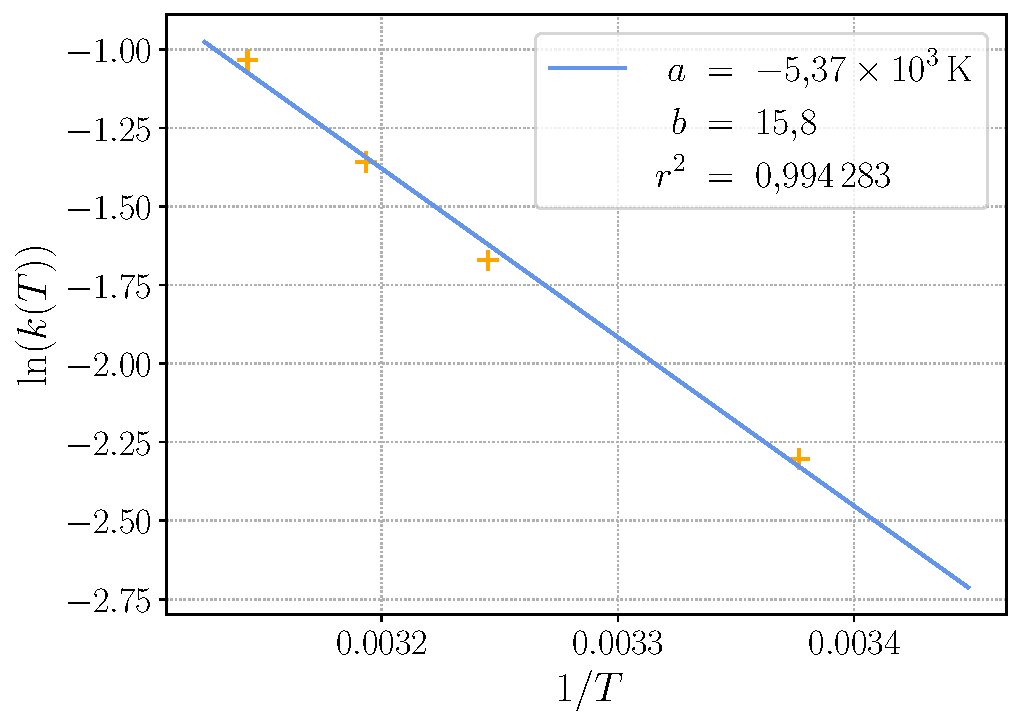
\includegraphics[width=\linewidth]{reglin_k}
		\end{center}
	\end{minipage}
}
\vspace{-15pt}

\end{document}
